\documentclass{beamer}
\usepackage{amssymb}
\usepackage{listings}
\usetheme{Berlin}
\usecolortheme{beaver}
\usefonttheme{structuresmallcapsserif}

\AtBeginSection[]
{
    \begin{frame}
      \frametitle{Table of Contents}
      \tableofcontents[currentsection]
    \end{frame}
}

\title{Introduction to Cryptography 1}
\subtitle{Definitions and Introduction to Substitution Ciphers}
\author{Yicheng Wang}
\institute{White Hat Academy}
\date{2015-03-06}
\subject{Computer Science}

\definecolor{codegreen}{rgb}{0,0.6,0}
\definecolor{codegray}{rgb}{0.5,0.5,0.5}
\definecolor{codeblue}{rgb}{0,0,0.6}
\definecolor{backcolor}{rgb}{0.95,0.95,0.95}

\lstdefinestyle{mystyle}{
	backgroundcolor = \color{backcolor},
	commentstyle = \color{codeblue},
	keywordstyle = \color{codegreen},
	numberstyle = \color{codegray},
	stringstyle = \color{magenta},
	basicstyle = \tiny\ttfamily,
	breakatwhitespace = false,
	breaklines = true,
	captionpos = b,
	keepspaces = true,
	numbers = left,
	numbersep = 5pt,
	showspaces = false,
	showstringspaces = false,
	showtabs = false,
	tabsize = 4
}

\lstset{style = mystyle}


\begin{document}

\frame{\titlepage}

\begin{frame}
\begin{itemize}
    \frametitle{What is Cryptography?}
    \item Cryptography is the study of encodings.
    \item Cryptographic algorithms are the algorithms used to encode messages
        such as "Hello World" into "b10a8db164e0754105b7a99be72e3fe5."
    \item Some necessary definitions:
        \begin{itemize}
            \item Plaintext (message): the original message.
            \item Key: the encryption/decryption agent (sometimes
                non-existent).
            \item Ciphertext: the result of a crypto algorithm.
        \end{itemize}
    \end{itemize}
\end{frame}

\begin{frame}
    \begin{itemize}
    \item Any cryptographic algorithm has an inverse with respect to the
        plaintext, the original function is called the encryption algorithm and
        the inverse is called the decryption algorithm.
    \item Good cryptographic algorithms are bijective with respect to the
        plaintext message, which means that each ciphertext is unique to a
        message-key pair.
    \item In mathematical terms:
        \[
            \exists Encryption: \{Plaintext\} \times \{Keys\} \to \{Ciphertext\}
        \]
        \[
            \exists Decryption: \{Ciphertext\} \times \{Keys\} \to \{Plaintext\}
        \]
\end{itemize}
\end{frame}

\begin{frame}
\frametitle{Why cryptography?}
\begin{itemize}
    \item Cryptography is very useful in our modern society, with the end of the
        age of privacy, everything one does on the internet is strictly
        monitored by everyone, thus the only way of protecting one's privacy is
        by encryption.
    \item Different algorithms offer different degrees of security, but some is
        still better than none.
\end{itemize}
\end{frame}

\begin{frame}
\frametitle{Substitution Ciphers}
\begin{itemize}
    \item One of the earliest forms of encryption is the substitution cipher. A
        substitution cipher is a method of encoding that divide the plaintext
        into pieces (most commonly letters) and substitute each piece with its
        corresponding ciphertext.
\end{itemize}
\end{frame}

\begin{frame}
    There are a lot of substitution ciphers. Their advantage lies in how easy it
    is to make them, but that also means that they are easily cracked. For this
    reason, a lot of substitution ciphers are not designed for security reasons
    but rather as a means to transmit data. Morse code is an example of this.

    \begin{figure}[h]
        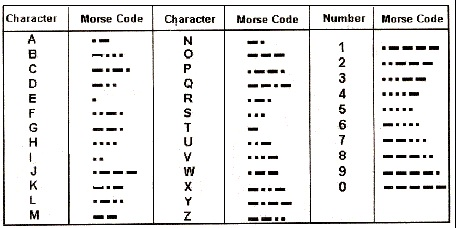
\includegraphics[width=0.7\textwidth]{morse-code-table}
    \end{figure}
\end{frame}

\begin{frame}
    \frametitle{Interpretation of Data}
    \begin{itemize}
        \item In cryptography, the most common ways of interpreting data is
            actually as numbers!
        \item For computers, numbers are easily manipulatable and there does
            exist a basic connection between numbers and strings, this is known
            as ASCII (American Standard Code for Information Interchange)
            encoding, as shown in the next slide.
    \end{itemize}
\end{frame}

\begin{frame}
    \frametitle{ASCII encoding}
    \begin{figure}[h]
        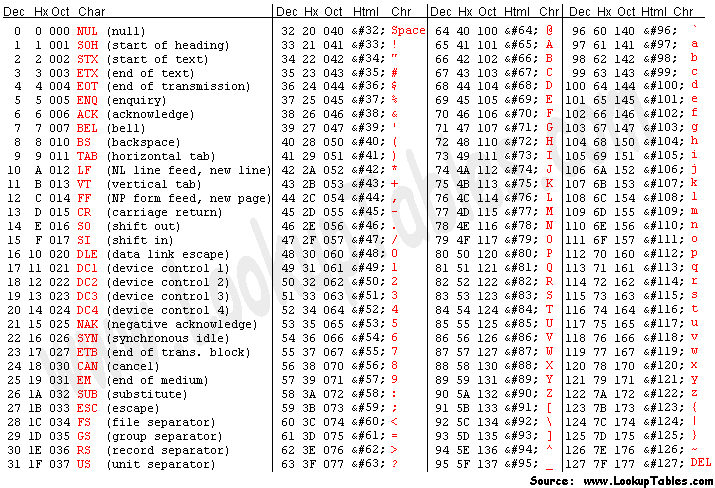
\includegraphics[width=0.9\textwidth]{asciifull}
    \end{figure}
\end{frame}

\begin{frame}

    One of the more ``useful'' ciphers out there is the rot-N cipher, or Cesser
    Shift. It takes the alphabet, shifts it N units forward and then overlays it
    with the original alphabet to create the substitution. rot-13 functions as
    follows:

    \begin{figure}[h]
        \begin{center}
            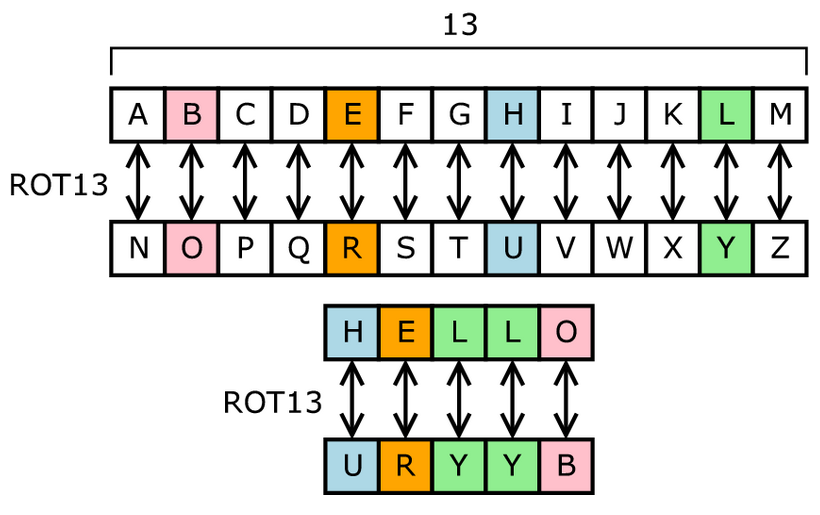
\includegraphics[width=0.5\textwidth]{ROT13}
        \end{center}
        \caption{Credit goes to Matt Crypto of Wikipedia.}
    \end{figure}
\end{frame}

\begin{frame}[fragile]
\frametitle{ROT-13}

Following is a sample code for a rot-N algorithm.

\begin{lstlisting} [language=Python]
def encrypt(data, N):
    result = []
    for c in list(data):
        # Upper Case Letters
        if ord(c) > 64 and ord(c) < 91:
            result.append(chr(65 + (ord(c) - 65 + N) % 26))

        # Lower Case Letters
        if ord(c) > 96 and ord(c) < 123:
            result.append(chr(97 + (ord(c) - 97 + N) % 26))

        # We ignore everything else
        else:
            result.append(c)

    return "".join(result)
\end{lstlisting}

\end{frame}

\begin{frame}
\frametitle{Mono-alphabetic Substitution Ciphers}
What we just discussed is called a \textbf{mono-alphabetic} substitution cipher
because it uses the same encryption scheme for each letter.

Note that this is not particularly safe and can be easily broken, as long as one
has figured out the complete encryption table, one has cracked the entire
algorithm. The following is another rather old algorithm, let's see what it
does:
\end{frame}

\begin{frame}
    \frametitle{Challenge algorithm}

    You know that "the quick brown fox jumps over the lazy dog" encrypts to:

    \begin{center}
     tsv jfrxp yildm ulc qfnkh levi gsv ozab wlt 
    \end{center}

    Using that info, try to figure out what this means:

    uozt: gsrh\_rh\_gsv\_zgyzhs\_xrksvi 

    As an additional challenge, try to code it!
\end{frame}

\begin{frame}
    \frametitle{Plain-text Attack}
    \begin{itemize}
        \item What we just did was called a "plain-text attack" or a crib
            attack. It works because we knew a part of the text and then
            can use it to find the encryption algorithm.
        \item However, that raises the question of what if we don't know
            anything about the text?
        \item As an exercise: go to this url: http://tinyurl.com/encodedMsg
        \item Grab the file, it looks like gibberish, you know that it is an
            encryption based on monoalphabetic substitution... But what else do
            you know?
    \end{itemize}
\end{frame}

\end{document}
